\documentclass[tikz,border=5mm]{standalone}
\usepackage{xcolor}

\definecolor{gameblue}{RGB}{0, 102, 204}

\begin{document}
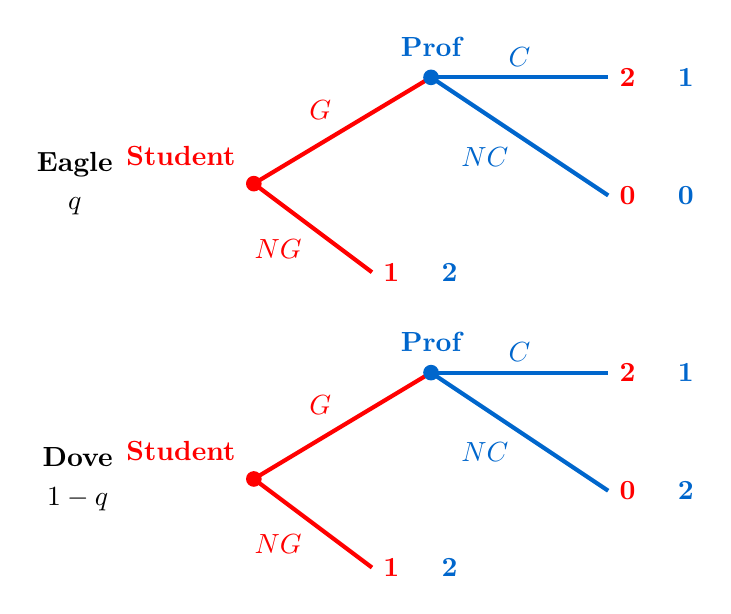
\begin{tikzpicture}[
    scale=1.5,
    font=\bfseries,
    dot/.style={circle, fill=#1, inner sep=2pt},
    dot/.default=black,
    line width=1.5pt
]

    % ==========================================
    % TOP TREE (Eagle / q)
    % ==========================================
    \coordinate (t_root)    at (0, 0);
    \coordinate (t_qg)      at (1.5, 0.9);
    \coordinate (t_ng)      at (1.0, -0.75);
    \coordinate (t_leaf_c)  at (3.0, 0.9);
    \coordinate (t_leaf_nc) at (3.0, -0.1);

    % Level 1 branches (Student - Red)
    \draw[red] (t_root) -- (t_qg) node[midway, above left] {$G$};
    \draw[red] (t_root) -- (t_ng) node[midway, below left] {$NG$};

    % Level 2 branches (Prof - Blue)
    \draw[gameblue] (t_qg) -- (t_leaf_c)  node[midway, above] {$C$};
    \draw[gameblue] (t_qg) -- (t_leaf_nc) node[midway, below left] {$NC$};

    % Nodes & Labels (Student placed 'above left', Eagle shifted further left)
    \node[dot=red, label={[red, anchor=south east]above left:Student}] at (t_root) {};
    \node[dot=gameblue, label={[gameblue]above:Prof}] at (t_qg) {};
    \node[align=center, anchor=east] at (-1.1, 0) {Eagle\\[2pt]$q$};

    % Payoffs (Red \quad Blue)
    \node[right] at (t_ng)      {\textcolor{red}{1} \quad \textcolor{gameblue}{2}};
    \node[right] at (t_leaf_c)  {\textcolor{red}{2} \quad \textcolor{gameblue}{1}};
    \node[right] at (t_leaf_nc) {\textcolor{red}{0} \quad \textcolor{gameblue}{0}};


    % ==========================================
    % BOTTOM TREE (Dove / 1-q)
    % ==========================================
    \coordinate (b_root)    at (0, -2.5);
    \coordinate (b_qg)      at (1.5, -1.6);
    \coordinate (b_ng)      at (1.0, -3.25);
    \coordinate (b_leaf_c)  at (3.0, -1.6);
    \coordinate (b_leaf_nc) at (3.0, -2.6);

    % Level 1 branches (Student - Red)
    \draw[red] (b_root) -- (b_qg) node[midway, above left] {$G$};
    \draw[red] (b_root) -- (b_ng) node[midway, below left] {$NG$};

    % Level 2 branches (Prof - Blue)
    \draw[gameblue] (b_qg) -- (b_leaf_c)  node[midway, above] {$C$};
    \draw[gameblue] (b_qg) -- (b_leaf_nc) node[midway, below left] {$NC$};

    % Nodes & Labels (Student placed 'above left', Dove shifted further left)
    \node[dot=red, label={[red, anchor=south east]above left:Student}] at (b_root) {};
    \node[dot=gameblue, label={[gameblue]above:Prof}] at (b_qg) {};
    \node[align=center, anchor=east] at (-1.1, -2.5) {Dove\\[2pt]$1-q$};

    % Payoffs (Red \quad Blue)
    \node[right] at (b_ng)      {\textcolor{red}{1} \quad \textcolor{gameblue}{2}};
    \node[right] at (b_leaf_c)  {\textcolor{red}{2} \quad \textcolor{gameblue}{1}};
    \node[right] at (b_leaf_nc) {\textcolor{red}{0} \quad \textcolor{gameblue}{2}};

\end{tikzpicture}
\end{document}
